\let\negmedspace\undefined
\let\negthickspace\undefined
\documentclass[journal]{IEEEtran}
\usepackage[a5paper, margin=10mm, onecolumn]{geometry}
%\usepackage{lmodern} % Ensure lmodern is loaded for pdflatex
\usepackage{tfrupee} % Include tfrupee package

\setlength{\headheight}{1cm} % Set the height of the header box
\setlength{\headsep}{0mm}     % Set the distance between the header box and the top of the text

\usepackage{gvv-book}
\usepackage{gvv}
\usepackage{cite}
\usepackage{amsmath,amssymb,amsfonts,amsthm}
\usepackage{algorithmic}
\usepackage{graphicx}
\usepackage{textcomp}
\usepackage{xcolor}
\usepackage{txfonts}
\usepackage{listings}
\usepackage{enumitem}
\usepackage{mathtools}
\usepackage{gensymb}
\usepackage{comment}
\usepackage[breaklinks=true]{hyperref}
\usepackage{tkz-euclide} 
\usepackage{listings}
% \usepackage{gvv}                                        
\def\inputGnumericTable{}                                 
\usepackage[latin1]{inputenc}                                
\usepackage{color}                                            
\usepackage{array}                                            
\usepackage{longtable}                                       
\usepackage{calc}                                             
\usepackage{multirow}                                         
\usepackage{hhline}                                           
\usepackage{ifthen}                                           
\usepackage{lscape}
\begin{document}

\bibliographystyle{IEEEtran}
\vspace{3cm}

\title{12.582}
\author{EE25BTECH11049 - Sai Krishna Bakki}
\maketitle
\vspace{-3em}
\textbf{Question:}\\
The position vector $OP$ of point $\vec{P}$ = (20,10) is rotated anti-clockwise in the X-Y plane by an angle $\theta=30^\degree$ such that point $\vec{P}$ occupies position $\vec{Q}$. The coordinates (x,y) of $\vec{Q}$ is \\
\solution\\
Given
\begin{align}
    \vec{P}=\myvec{20\\10},\theta&=30^\degree
\end{align}
we use
\begin{align}
    \vec{x_n}=\vec{R}\vec{x_o}
\end{align}
where $\vec{R}$ is Rotation matrix
\begin{align}
    \vec{Q}=\myvec{\cos\theta&-\sin\theta\\ \sin\theta&\cos\theta}\vec{P}\\
    \vec{Q}=\myvec{\cos30^\degree&-\sin30^\degree\\ \sin30^\degree&\cos30^\degree}\myvec{20\\10}\\
    \vec{Q}=\myvec{\frac{\sqrt{3}}{2}&\frac{-1}{2}\\\frac{1}{2}&\frac{\sqrt{3}}{2}}\myvec{20\\10}\\
    \vec{Q}=\myvec{10\sqrt{3}-5\\10+5\sqrt{3}}
\end{align}
Using approximation, the coordinates of $\vec{Q}$ is
\begin{align}
    \vec{Q}=\myvec{12.32\\18.66}
\end{align}
\newpage
\begin{figure}
    \centering
    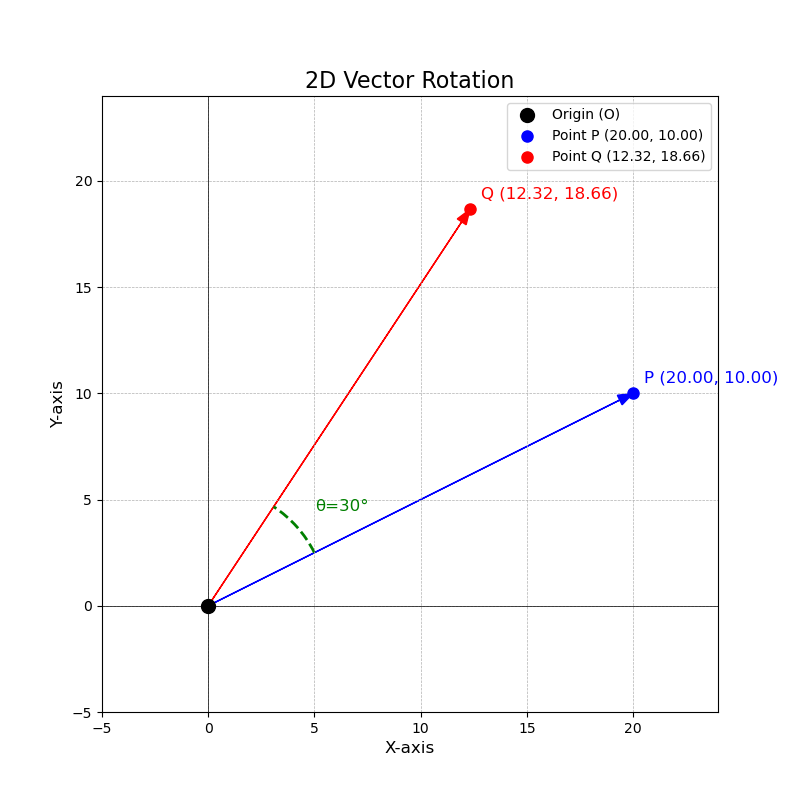
\includegraphics[width=1.1\columnwidth]{figs/Figure_1.png}
    \caption{}
    \label{fig:placeholder}
\end{figure}
\end{document}